\documentclass[11pt]{article}

\usepackage[a4paper,margin=2.2cm]{geometry}
\usepackage{xcolor}
\usepackage{booktabs}
\usepackage{listings}
\usepackage{enumitem}
\usepackage{tabularx}
\usepackage{titlesec}
\usepackage[hidelinks]{hyperref}
\usepackage{graphicx}
\usepackage{float}
\usepackage{subcaption}
\graphicspath{{figs/}}

\definecolor{accent}{HTML}{1F4E79}
\definecolor{soft}{HTML}{F4F1EA}
\definecolor{codebg}{HTML}{F7F7F4}
\definecolor{rule}{HTML}{B0392B}

\titleformat{\section}{\large\bfseries\color{accent}}{\thesection}{0.6em}{}
\titleformat{\subsection}{\normalsize\bfseries\color{accent}}{\thesubsection}{0.6em}{}

\lstset{
  basicstyle=\ttfamily\scriptsize,
  backgroundcolor=\color{codebg},
  breaklines=true, frame=single, rulecolor=\color{gray!40},
  numbers=left, numberstyle=\tiny\color{gray}, numbersep=6pt,
  keywordstyle=\color{accent}\bfseries, commentstyle=\color{gray!70}\itshape,
  stringstyle=\color{rule}, showstringspaces=false, language=Python,
  xleftmargin=2em, framexleftmargin=1.6em,
}

\newcommand{\code}[1]{\texttt{\small #1}}
% AUTO-GENERATED by gen_numbers.py from reports/results.json — do not edit.

\newcommand{\nReports}{12}
\newcommand{\nFiles}{12}
\newcommand{\coverageRate}{100\%}
\newcommand{\primaryFieldAcc}{100\%}
\newcommand{\primaryFieldsCorrect}{24}
\newcommand{\primaryFieldsTotal}{24}
\newcommand{\primaryReportAcc}{100\%}
\newcommand{\primaryMAE}{0.0}
\newcommand{\baselineFieldAcc}{87.5\%}
\newcommand{\fieldAccGain}{12.5\%}
\newcommand{\alertTP}{1}
\newcommand{\alertFP}{0}
\newcommand{\alertFN}{0}
\newcommand{\alertPrecision}{100\%}
\newcommand{\alertRecall}{100\%}
\newcommand{\baselineRecall}{0\%}
\newcommand{\expectedAlerts}{NA-CHI-021}
\newcommand{\predictedAlerts}{NA-CHI-021}
\newcommand{\baselineMissed}{NA-CHI-021}
\newcommand{\meanConfidence}{96.5\%}
\newcommand{\reviewRate}{25\%}
\newcommand{\reportsFlagged}{3}
\newcommand{\flaggedSites}{EU-PL-005, NA-AUS-009, NA-CHI-021}
\newcommand{\baselineAgreement}{87.5\%}
\newcommand{\meanLatency}{0.01}
\newcommand{\throughput}{76,244}
\newcommand{\costNote}{offline mock — no API calls, \$0}
\newcommand{\nTests}{86}
\newcommand{\runMode}{mock}


\title{\vspace{-1.2cm}\color{accent}\bfseries Quality-Control Pipeline\\[2pt]
\large\mdseries A mini agent that reads inspection reports, flags defect breaches,\\and measures how well it does its own job}
\author{Alex Huou}
\date{\today}

\begin{document}
\maketitle
\vspace{-0.8cm}

\begin{center}\fcolorbox{accent}{soft}{\parbox{0.95\linewidth}{\small
\textbf{Executive summary.} This tool reads manufacturing inspection reports, uses a
language model to pull defect counts out of free-text inspector notes, and emails
operations when a facility exceeds its quality limits. On the \nReports{} sample
reports it read \primaryFieldsCorrect{} of \primaryFieldsTotal{} defect counts
correctly (\primaryFieldAcc), correctly flagged the \alertTP{} facility that breached
limits with \alertFP{} false alarms, and ran in milliseconds at zero cost. Crucially,
the system \emph{measures its own reliability} in plain terms a manager can act on ---
how accurately it reads, how confident it is, when it asks a human to double-check, and
what it would cost at scale --- so the people relying on it can see exactly how far to
trust it.
}}\end{center}

\medskip
\noindent\textbf{One report --- NA-CHI-021 --- exercises everything this brief asks for; \S4 walks it end to end.}
Where each requirement is demonstrated:

\begin{center}\small
\begin{tabularx}{\linewidth}{@{}l X@{}}
\toprule
\textbf{What you asked for} & \textbf{Where it's shown}\\
\midrule
Explore \& understand unfamiliar data & \S1 --- the report schema and the free-text extraction problem\\
Data extraction with modern techniques & \S1--\S2, \S5 --- LLM structured-output extraction, robust to unseen phrasing\\
Clean, readable, testable code & \S6 + Appendix B --- pluggable modules, a pure rules engine, \nTests{} tests\\
Explainability to non-technical audiences & \S3 --- the tool-quality metrics table\\
Logical problem-solving & \S4 --- the ``13 hundred'' case study; \S5 --- adversarial hardening\\
\bottomrule
\end{tabularx}
\end{center}

\section{The problem, and why a language model}
Each inspection report is a JSON file with hard production numbers plus two
\emph{free-text} notes written by a human auditor --- one for major (critical) defects,
one for minor (cosmetic) defects. The task is to alert stakeholders when defects exceed
the limits:

\begin{center}\small
major $> 1\%$ \quad$\bullet$\quad minor $> 3\%$ \quad$\bullet$\quad (major + minor) $> 3.5\%$
\quad of total production.
\end{center}

The numbers are trivial to threshold; the hard part is \emph{reading the counts out of
prose that varies every time}. Across the sample alone the auditors wrote
``\,\code{31 units}\,'', ``\,\code{a dozen}\,'' (12), ``\,\code{half a dozen}\,'' (6),
``\,\code{a hundred}\,'' (100), ``\,\code{a single unit}\,'' (1), ``\,\code{None}\,'' (0),
and the decisive ``\,\code{13 hundred units}\,'' (1300). A regular expression that grabs
the first integer reads ``13 hundred'' as \textbf{13} --- and that one misread is the
difference between catching and missing the only true breach in the dataset. This is
exactly why the brief calls for an LLM: the reading problem is open-ended natural
language, not a fixed pattern.

\section{How it works}
The pipeline is five small, independently testable stages:

\begin{enumerate}[leftmargin=1.4em,itemsep=2pt]
  \item \textbf{Load} every report and pull out the production total and the two notes
    (\code{loader.py}), degrading gracefully --- a malformed file becomes a recorded
    coverage gap, never a crash.
  \item \textbf{Extract} the major/minor counts from the notes behind a pluggable
    \code{Extractor} interface. In \textbf{live} mode an Anthropic model returns a
    \emph{structured} result (forced JSON schema); in \textbf{mock} mode a deterministic,
    offline parser stands in so the whole system runs with no API key at \$0.
  \item \textbf{Cross-check} every reading against an independent, deliberately naive
    rule-based reader. Where they disagree, the report is flagged for a human.
  \item \textbf{Decide} via the pure threshold engine (\code{rules.py}; strict $>$ at
    every boundary).
  \item \textbf{Alert} stakeholders with a plain-language email (\code{alerting.py},
    stubbed), and \textbf{measure} the tool's own quality into \code{results.json}.
\end{enumerate}

\noindent The mock extractor is \emph{not} a lookup table of the sample answers --- it
runs the same robust number-reading logic (\code{number\_words.py}) the live model is
prompted to emulate, so it generalises to unseen wording. That is what lets us measure
the tool honestly offline and ship something reproducible.

\section{Measuring the tool (the part that matters)}
The metrics below grade \emph{the agent}, not the factory. They are deliberately not
defect rates --- they answer ``how much can we trust what this tool tells us?''. Every
number is generated from a real run (\code{results.json}); none is hand-typed.

\begin{center}\small
\begin{tabularx}{\linewidth}{@{}l l X@{}}
\toprule
\textbf{Question} & \textbf{Result} & \textbf{What it means for a non-technical reader}\\
\midrule
Did it read the counts right? & \primaryFieldAcc & Read \primaryFieldsCorrect/\primaryFieldsTotal{} defect counts correctly; average error \primaryMAE{} units.\\[2pt]
Does the LLM earn its keep? & +\fieldAccGain & A rules-only reader gets \baselineFieldAcc{} and \emph{misses the breach} at \baselineMissed.\\[2pt]
Did it catch the breaches? & \alertRecall{} recall & Flagged \alertTP/\alertTP{} real breach(es), \alertFP{} false alarms (precision \alertPrecision).\\[2pt]
How sure was it? & \meanConfidence & Mean confidence across all readings; low-confidence reads are auto-flagged.\\[2pt]
How often ask a human? & \reviewRate & \reportsFlagged{} of \nReports{} reports flagged for a quick human check.\\[2pt]
How fast? & \meanLatency~ms & Per report in offline mock; live throughput is set by the model call ($\sim$1--2\,s each, run concurrently).\\[2pt]
What does it cost? & \$0 & \costNote.\\[2pt]
Did it read every file? & \coverageRate & \nFiles/\nFiles{} report files read without error.\\
\bottomrule
\end{tabularx}
\end{center}

\noindent\textbf{Why a cross-check, and why ``ask a human''.} The tool runs a second,
intentionally simple reader alongside the main one. The two agree on \baselineAgreement{}
of readings; the \reportsFlagged{} disagreements (\flaggedSites) are surfaced for review.
This is conservative by design: in a safety setting it is far better to ask an operator to
glance at a report than to silently trust an automated read --- and, satisfyingly, the one
true breach is among the flagged reports, so a human is asked to confirm it.

\section{Case study: ``13 hundred''}
Report \code{NA-CHI-021} produced 6{,}100 units; its minor-defect note reads
\emph{``13 hundred units exhibited slight connector misalignment.''} The tool reads
\textbf{1{,}300} (21.3\% of production), which trips both the minor ($>3\%$) and overall
($>3.5\%$) rules, and emails operations. The naive cross-check reads \textbf{13} (0.2\%)
and would have stayed silent --- a missed breach. The pipeline (i) gets it right, (ii)
shows \emph{why} (it quotes the snippet ``13 hundred'' as evidence in the alert), and
(iii) flags the report for human confirmation because its two readers disagreed. One case,
all three behaviours the brief is really asking for.

\section{Robustness, and not overfitting}
The brief warns that real notes will be worded differently from the sample, so the system
is built to generalise and was then \emph{adversarially stress-tested}:

\begin{itemize}[leftmargin=1.4em,itemsep=2pt]
  \item The number reader composes compound numerals left-to-right, so unseen phrasings
    read correctly: ``sixty five'' $\to$ 65, ``two hundred and fifty'' $\to$ 250,
    ``twenty-five hundred'' $\to$ 2500, ``a couple dozen'' $\to$ 24, ``1.5k'' $\to$ 1500.
    Vague quantifiers (``a few'', ``several'') are read but kept at low confidence so they
    route to a human rather than passing as fact.
  \item A panel of independent reviewers tried to break each component (the parser, the
    rules, the metrics, the offline guarantee, the tests). They confirmed the core
    contract and surfaced real gaps --- most importantly that an earlier version misread
    spelled-out compounds like ``sixty five'' as 5 at high confidence (a silent
    under-count), and that a failed read on a breach was being scored as a clean run.
    Both are fixed and now covered by tests.
\end{itemize}

\section{Engineering notes}
\begin{itemize}[leftmargin=1.4em,itemsep=2pt]
  \item \textbf{Modular \& testable.} Pure threshold engine (no I/O), a pluggable
    \code{Extractor} interface (mock / live / baseline), and a metrics layer with a
    hand-verified golden set. \nTests{} automated tests pass, including the ``13 hundred''
    trap, every threshold boundary, the synthetic major-only / overall-only cases, an
    offline ``no API key'' proof, and a failed-read-on-the-breach safety test.
  \item \textbf{Live integration.} The live extractor uses Anthropic structured outputs
    (a forced schema), reads its key from the environment, and reports token usage so the
    tool can show an illustrative cost-per-report. It is drop-in: the mock and live paths
    share one interface, and the live path is unit-tested with a fake client.
  \item \textbf{Runs anywhere, \$0.} \code{python -m qc\_pipeline --mode mock} needs only
    \code{pydantic}; the Anthropic SDK is imported lazily and only for live mode.
  \item \textbf{Optional operator console.} A small FastAPI dashboard (\code{webapp/}) wraps
    the pipeline for non-technical users --- mock/live runs, an e-mail outbox, a raw-report
    viewer, and a content-hash cache that avoids re-spending tokens on unchanged reports
    (\S\ref{sec:console}). The CLI and test suite are the deliverable; the console is additive.
\end{itemize}

\section{The operator console (web app)}\label{sec:console}
The deliverable is the CLI and test suite; layered on top is a small FastAPI dashboard
(\code{webapp/}, also deployed live\footnote{\href{https://mini-agent-qc.vercel.app}{\nolinkurl{mini-agent-qc.vercel.app}} --- the offline analysis runs on load at \$0; live extraction is optional and runs on a budgeted demo key or your own.})
that lets a non-technical operator \emph{watch} the pipeline work: run it in mock or live mode,
see every tool-quality metric update, drag in new reports, and --- the two views below --- track what
the tool would send and inspect exactly what tripped an alert.

\paragraph{E-mail outbox.} The stubbed \code{send\_email()} (\code{alerting.py}) surfaces as a
tracker (Fig.~\ref{fig:outbox}): each breach becomes a \textsc{sent} alert and each review-flagged
report a \textsc{draft}, every one openable to read the exact rendered message (Fig.~\ref{fig:email}).
The body is an editable template, so an operator can tune the wording without touching code. Nothing is
actually e-mailed --- the stub logs the message --- and the panel says so explicitly, so the demo can
never be mistaken for live sending.

\paragraph{Report viewer.} Clicking an alert (or any ledger row) opens the underlying inspection JSON
with the decision-relevant fields highlighted (Fig.~\ref{fig:viewer}): the production total and the two
free-text notes. For \code{NA-CHI-021} the highlighted minor note --- \emph{``13 hundred units\dots''}
--- is the whole story: the tool read 1{,}300, the naive cross-check read 13, and the panel surfaces
both so a human can confirm in seconds. A file that fails to parse opens the same way with the offending
field flagged, making the ``coverage gap, not a crash'' behaviour visible rather than buried in a log.

\begin{figure}[H]
\centering
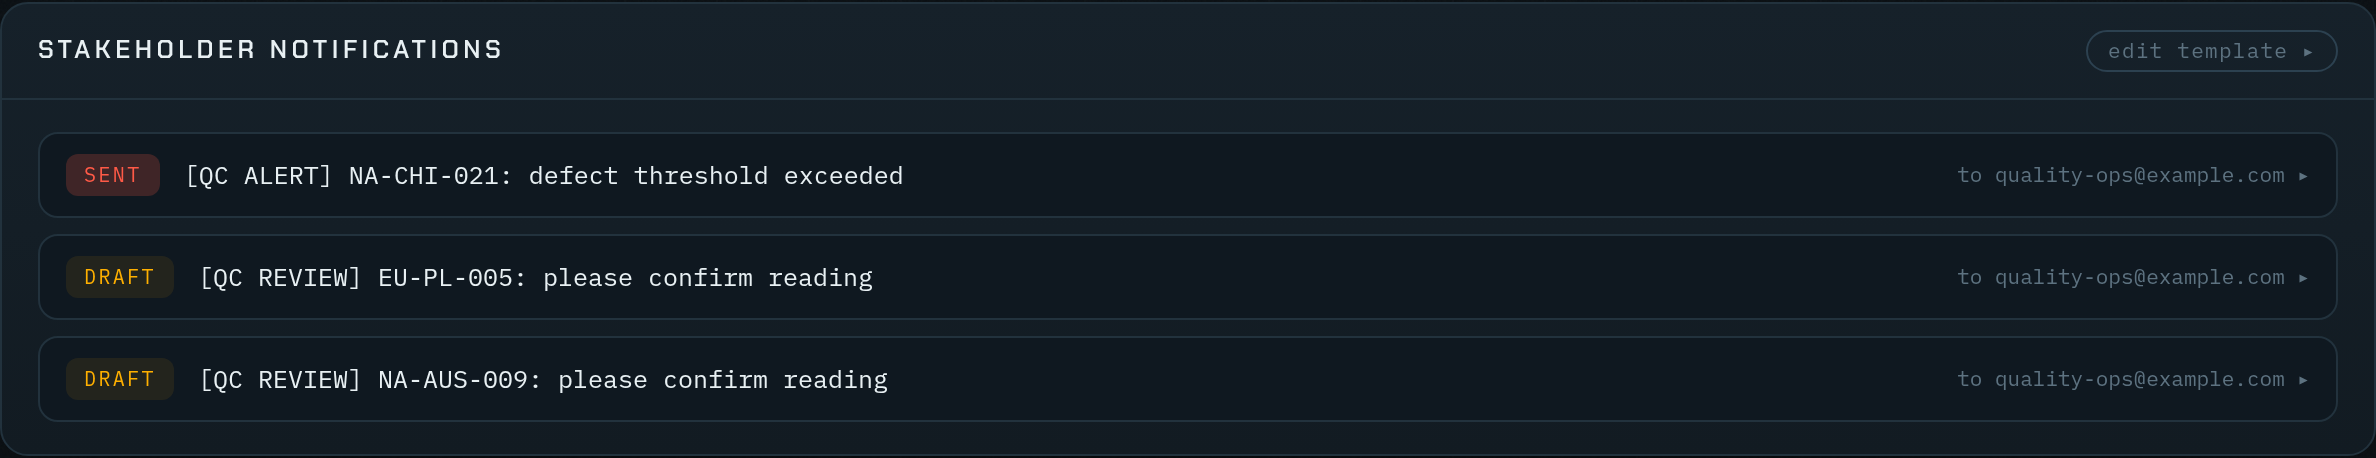
\includegraphics[width=\linewidth]{console_outbox.png}
\caption{The outbox turns the \code{send\_email()} stub into something a manager can see: the one breach
(NA-CHI-021) is a \textsc{sent} alert; the two reports the readers disagreed on are \textsc{draft} review
requests. Nothing leaves the machine.}
\label{fig:outbox}
\end{figure}

\begin{figure}[H]
\centering
\begin{subfigure}[t]{0.55\linewidth}
  \centering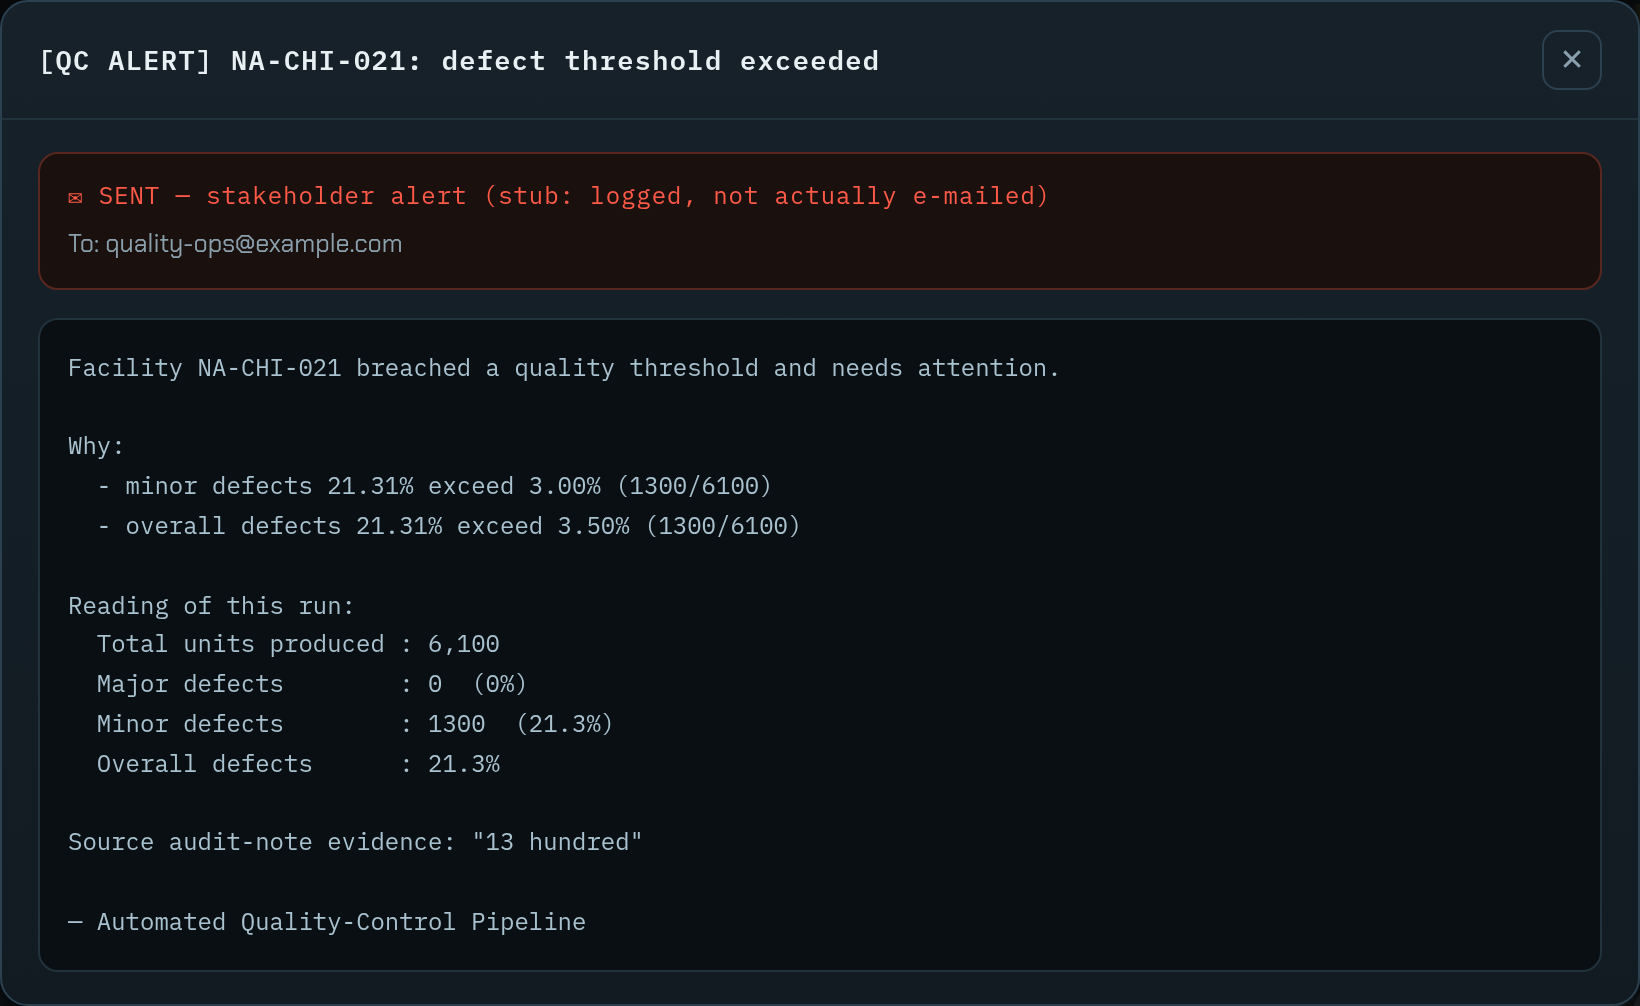
\includegraphics[width=\linewidth]{console_email.png}
  \caption{The rendered alert e-mail: a plain-language ``why'', the reading, and the quoted evidence
  ``13 hundred''. The header marks it a logged stub, not a sent message.}
  \label{fig:email}
\end{subfigure}\hfill
\begin{subfigure}[t]{0.42\linewidth}
  \centering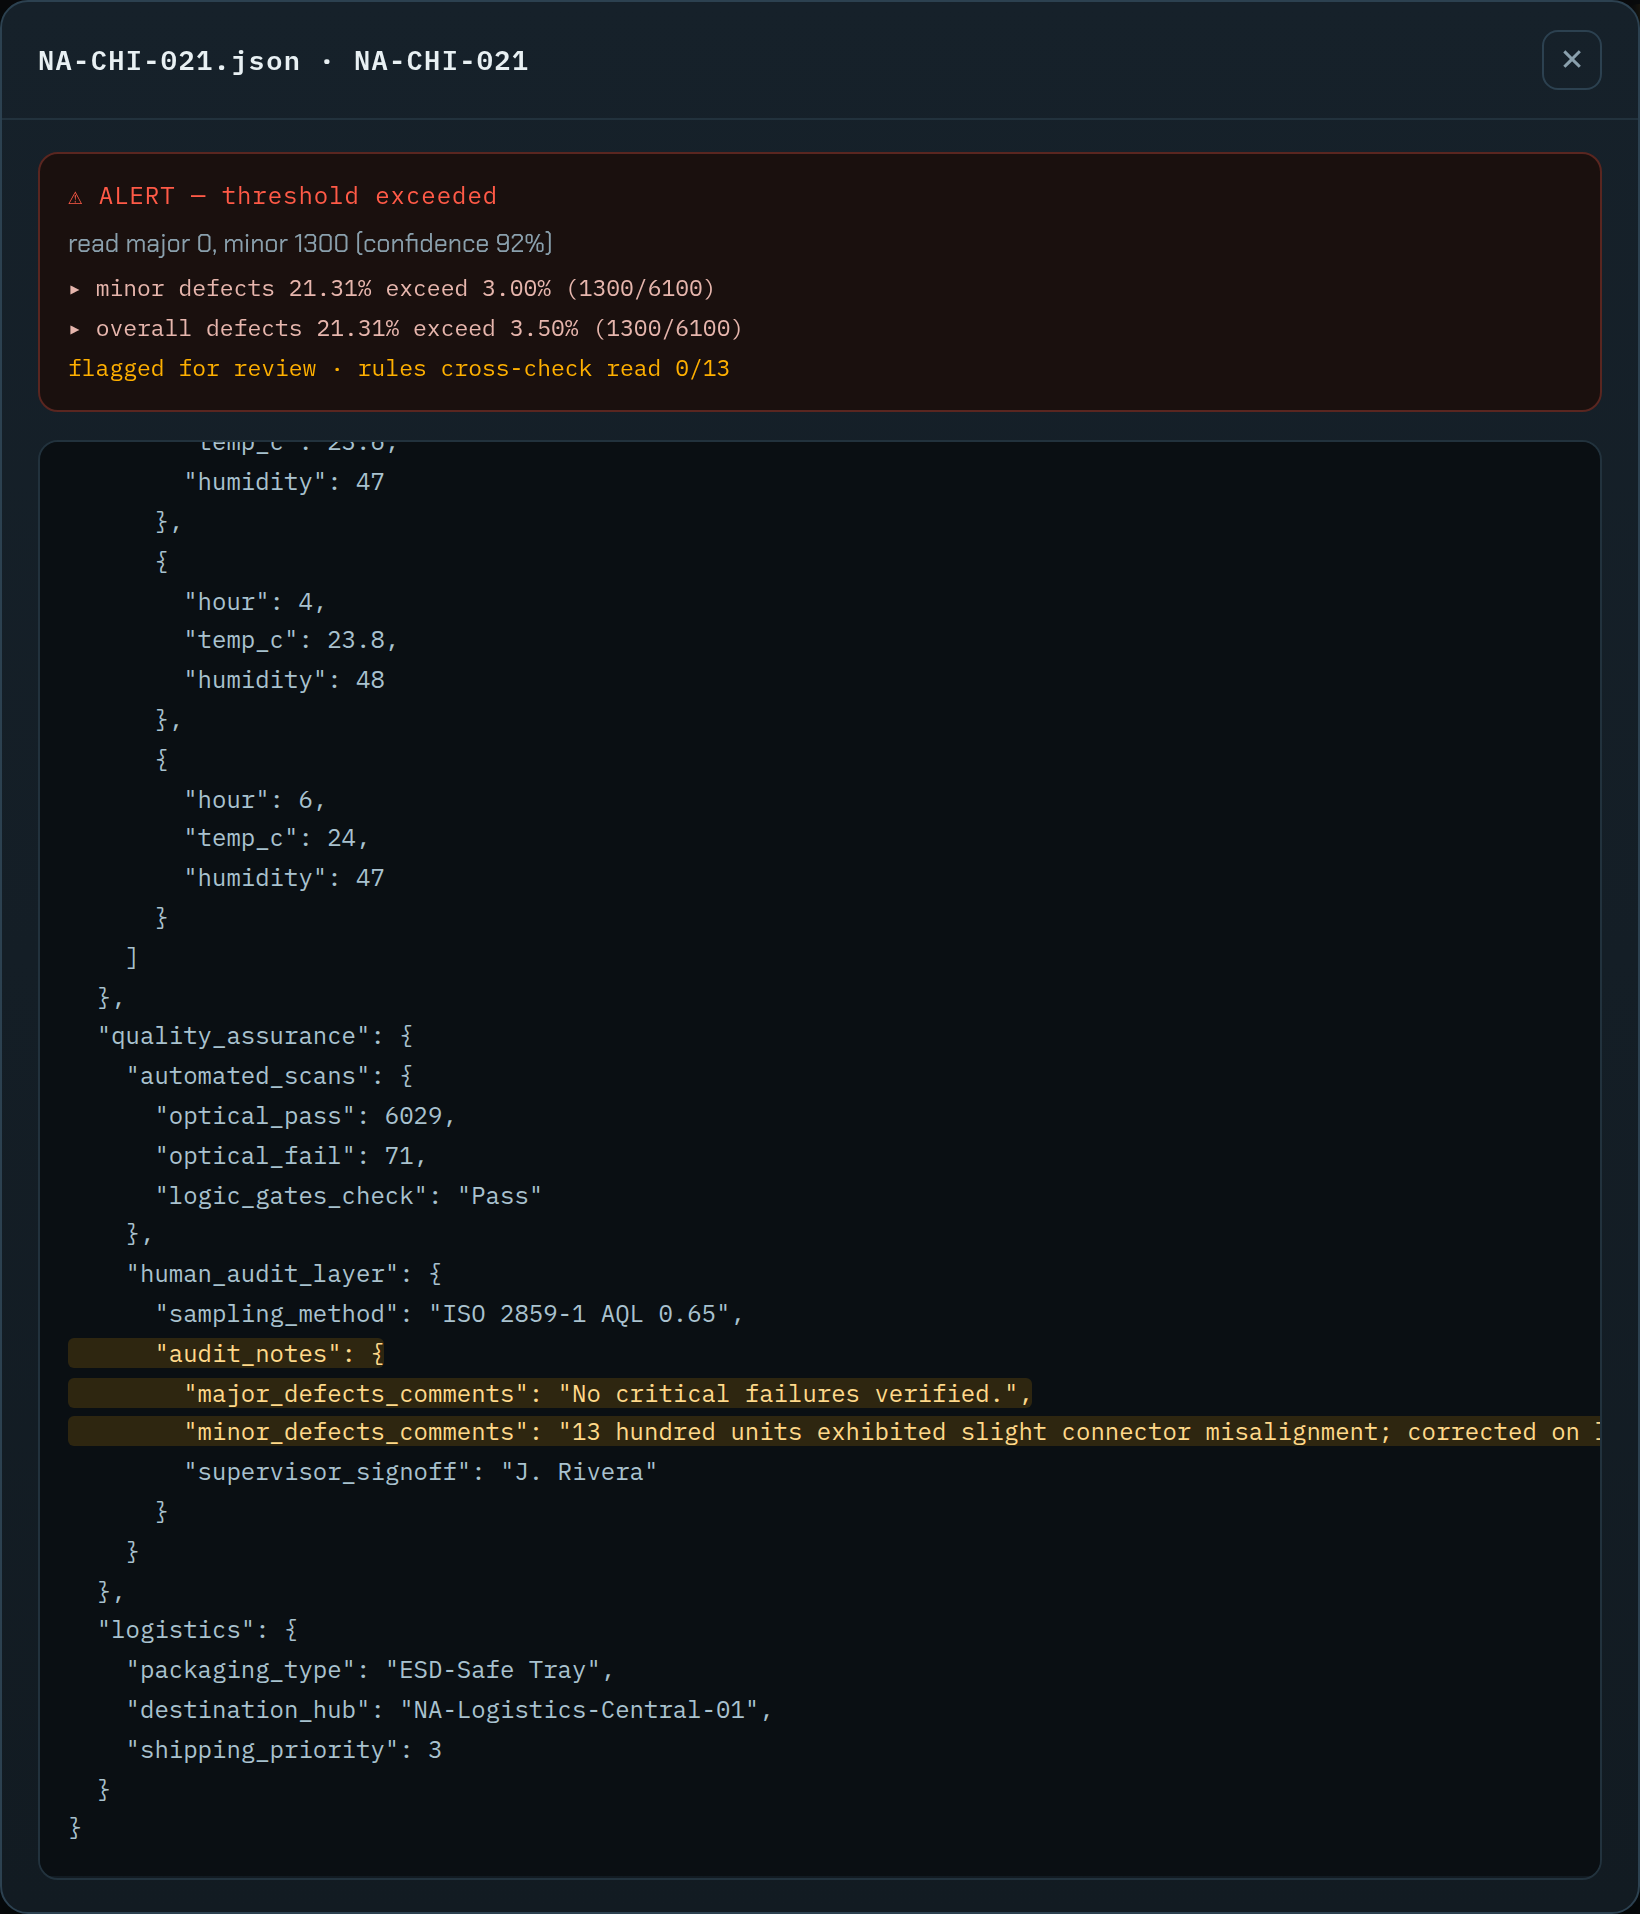
\includegraphics[width=\linewidth]{console_viewer_notes.png}
  \caption{The raw-JSON viewer with the total and the two audit notes highlighted --- the minor note
  ``13 hundred units\dots'' is what drives the breach.}
  \label{fig:viewer}
\end{subfigure}
\caption{Click an alert to see what the tool would send (left) and what tripped it (right).}
\label{fig:emailviewer}
\end{figure}

\section{Limitations \& future work}
The offline parser is a faithful but bounded stand-in for the model: it reads the first
quantity in a note (fine for single-count notes, ambiguous if a note mixes several
numbers), and treats vague quantifiers as low-confidence estimates. The golden set is the
12 provided reports; on genuinely new data the tool still reports confidence, speed,
coverage and alerts, but cannot score its own accuracy without labels. Natural extensions:
a small human-labelled validation set refreshed periodically, per-line-item extraction
when notes carry multiple counts, and trend dashboards across runs.

\appendix
\section{Running it}
\begin{lstlisting}[language=bash,numbers=none]
pip install -r requirements.txt
python -m qc_pipeline --mode mock      # offline, deterministic, $0
python -m pytest -q                    # full test suite

# Live (real model extraction):
cp .env.example .env                   # set ANTHROPIC_API_KEY
python -m qc_pipeline --mode live --tier balanced   # cheap=Haiku / balanced=Sonnet / max=Opus
\end{lstlisting}

\section{Key source: the number reader and the rules engine}
\lstinputlisting[caption={qc\_pipeline/extraction/number\_words.py — robust natural-language quantity parser}]{../qc_pipeline/extraction/number_words.py}
\lstinputlisting[caption={qc\_pipeline/rules.py — the pure defect-threshold engine}]{../qc_pipeline/rules.py}

\end{document}
